\section{Preliminary results}
\label{sec:results}

\begin{figure}
  \centering
  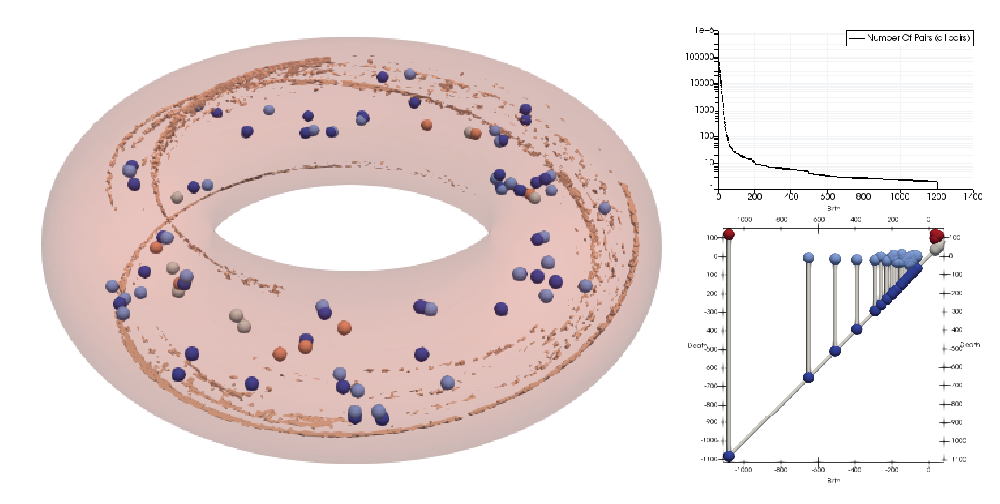
\includegraphics[width=\linewidth]{Figs/simplification3D}
  \caption{3D Visualization of a XGC simulation dataset: (a) the spatial view, (b) the persistence curve, (c) the persistence diagram.}
  \label{fig:results}
\end{figure}


%\begin{figure}[!htb]
%  \centering
%  \includegraphics[width=\linewidth]{Figs/results}
%  \caption{Preliminary results: (a) the 2D triangular mesh; (b) critical points extracted in a slice.}
%  \label{fig:results}
%\end{figure}

The visualization results shown in Figure~\ref{fig:results} have three views: the spatial view, the persistence curve, and the the persistence diagram.  

{\bf The spatial view} visualizes the spatial distribution of critical points and segmentations.  The critical points are visualized as spheres, and the colors encode the critical point types.  The figure also highlights one of the blobs (the dark yellow ribbons) that are extracted. 

{\bf The persistence curve} provides a visual hint for choosing the persistence threshold for topology simplification.  In this plot, the $x$-axis is the persistence threshold and the $y$-axis is the number of arcs or segmentations in the results.  Users can interactively choose the defined number of segmentations and thus define thresholds for different topology simplification results.  

{\bf The persistence diagram}~\cite{EdelsbrunnerLZ02} visualizes the critical point pair of each arc, and the diagram also serves as a visual hint for choosing proper persistence threshold.  The lower ($x$-axis) and upper ($y$-axis) values of each arc is plotted as a stem in the diagram.  The longer the stem, the higher persistent the arc.  Users can further investigate the simplification results by choosing different persistence thresholds.  

% The persistence plot is a 
% \remark{A persistence diagram is a scatter plot where each critical point pair is drawn as a point using the begin and end time as x, y coordinates. A pair's persistence is thus indicated by the vertical distance to the main diagonal.}

% We are already able to extract critical points in individual slices.  We will associate these points across different slices and timesteps for the next milestones.  We are also going to incorporate the RPCA into the workflow to simplify the input data.  We would also like to have discussions with fusion scientists to evaluate our approach.  

% Persistent diagram 

% Contour tree instead of Reeb graphs.  